\section{Skaitmeninės tapatybės valdymo apžvalga}

\subsection{Tapatybės patvirtinimo poreikis}

Šiais laikais naudotojo identifikavimas yra svarbi interneto taikomųjų
programų dalis. Paslaugų tiekėjai identifikuoja savo naudotojus norėdami \cite{RalucaBudiu2014}:

\begin{itemize}
    \item registruoti (angl. \textit{log}) naudotojų veiklą,
    \item užtikrinti, kad naudotojas iš tikrųjų yra asmuo, kuris sakosi esąs,
    \item suteikti dalį funkcionalumo tik autorizuotiems naudotojams,
    \item individualizuoti tinklalapio ar taikomosios programos turinį pagal naudotojo poreikius,
    \item sukurti paslaugos naudotojų bendruomenę,
    \item išvengti galimų anoniniminių naudotojų atakų.
\end{itemize}

Dėl išvardytų priežasčių naudotojų identifikavimas atlieka svarbią rolę įvairiose taikomųjų programų
srityse - elektroninėje valdžioje, elektroninėje komercijoje, verslo sumanume
(angl. \textit{business intelligence}), tyrimuose bei saugume
(angl. \textit{homeland security}) \cite{Glasser2009}. Kiekvienas paslaugų tiekėjas turi pasirinkti,
kaip autentifikuoti, ir, jei reikia, autorizuoti naudotojus. Programos kūrėjas taip pat turi saugoti
naudotojų suteiktus asmens duomenis ir užtikrinti jų saugumą, o naudotojui tenka rūpintis skirtingų turimų
paskyrų priežiūra ir savo duomenų sklaida tarp skirtingų sistemų. Minimus tapatybės atpažinimo
skaitmeninėje erdvėje aspektus nagrinėja skaitmeninės tapatybės valdymo disciplina.

\subsection{Skaitmeninės tapatybės valdymo samprata}

Dėl nuolat vykstančios interneto ir jame esančių paslaugų plėtros tapatybių
valdymo uždavinys pastaraisiais metais tapo itin svarbus \cite{Glasser2009}. Sprendžiant šį iššųkį,
sukurta skirtingų skaitmeninės tapatybės valdymo sistemų, siekiančių išspręsti naudotojų
tapatybės atpažinimo problemas. Šioms sistemoms įtaką daro
kiti tapatybę nagrinėjantys mokslai (pvz. sociologija), taip pat jos gali atlikti keletą skirtingų funkcijų, susijusių
su naudotojų tapatybe. Žemiau pateikiama diagrama,
kurioje pavaizduotas tapatybės valdymo sistemų kontekstas bei pagrindinės atliekamos užduotys:

\begin{figure}[H]
    \centering
    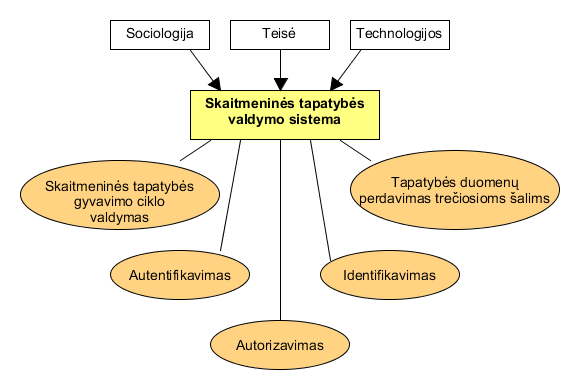
\includegraphics[scale=0.8]{img/IDMcontextAndUsecases}
    \caption{Skaitmeninių tapatybių valdymo sistemų kontekstas ir užduotys \cite{Glasser2009}}
\end{figure}

Paveiksle matomos disciplinos turi skirtingą poveikį tapatybių valdymo sistemoms. 
Sociologija padeda apibrėžti tapatybę ir jos atitikmenį skaitmeninėje erdvėje, teisės mokslas nusako tapatybės duomenų naudojimo reikalavimus,
o esamos technologijos formuoja sistemos įgyvendinimo niuansus. Verta pastebėti, kad tapatybės valdymo sistema gali atlikti ne visas
diagramoje nurodomas funkcijas, o tik dalį iš jų. Taip pat, 1-ame paveiksle bei visame darbe naudojamos skaitmeninės tapatybės valdymo sąvokos,
tokios kaip \textit{identifikavimas}, \textit{autentifikavimas} ar \textit{autorizavimas} neretai suprantamos skirtingai, o tai sukelia
vieningos terminologijos trūkumą ir dėl jo kylančius neaiškumus \cite{Glasser2009}. Dėl to skyriuje
\enquote{Sąvokų apibrėžimai} pateikiami darbe dažniausiai naudojamų terminų aiškinimai.

Esamų tapatybių valdymo sistemų architektūros bei veikimo principai yra skirtingi -  S. Clauß ir M.Köhntopp savo tyrime pastebi,
kad nėra vieningo standarto identiteto
valdymo sistemoms \cite{Claus2001}. Tolesniuose skyriuose, apžvelgus naudotojų bei paslaugų tiekėjų reikalavimus
tapatybės valdymo sistemoms, pateikiamos skirtingos technologijos
bei sprendimai, naudojami identiteto valdymui internete, jų privalumai bei trūkumai.

\subsection{Skaitmeninės tapatybės valdymo sistemų charakteristikos}

Šiame darbe į skaitmeninių tapatybių valdymą žvelgta iš dviejų perspektyvų: naudotojo bei paslaugų tiekėjo \textcolor{red}{palikt tik naudotojo?}. Abi pusės,
priklausomai nuo savo poreikių, iškelia jiems aktualias identiteto valdymo sistemų savybes. Darbe nagrinėjant skirtingas tapatybės valdymo sistemas,
didžiausias dėmėsys kreiptas į žemiau aprašytus naudotojams bei paslaugų tiekėjams svarbius sistemų bruožus.

Tiek naudotojams, tiek paslaugų tiekėjams itin svarbus yra pasirinkto identiteto valdymo sprendimo patikimumas, t.y., asmens duomenų saugumo užtikrinimas.
Naudotojai nenori savo asmens duomenų nutekėjimo (angl. \textit{data leakage}) internete, tuo tarpu paslaugų tiekėjai negali rizikuoti prarasti naudotojų pasitikėjimo
jų paslauga pasirinkus nesaugų tapatybės valdymo sprendimą. Be patikimumo, naudotojams bei paslaugų tiekėjams aktualios ir 
kitos skaitmeninio identiteto sistemų savybės. Žemiau pateikiami pagrindiniai abiejų pusių poreikiai.
\\

\chapter{\textbf{Naudotojams svarbūs tapatybės valdymo sistemų bruožai:}}

\begin{itemize}
    \item identifikatorių kiekis. Naudotojui vidutiniškai turint 25 paskyras, reikalaujančias slaptažodžių \cite{Florencio2007} bei naudojant
    nuo 2 iki 12-os el. paštų \cite{Gross2007} naudotojai tampa priversti prisiminti vis daugiau identifikatorių. Tai verčia naudotojus aukoti saugumą dėl patogumo ir naudoti panašius
    slaptažodžius skirtingose sistemose \cite{Pashalidis2003, Samar1999};
    \item asmens duomenų kontrolė. Pasak Nyderlanduose atliktų tyrimų, naudotojai jaučia, kad nekontroliuoja savo asmens duomenų internete \cite{Baars2016}. Dėl to
    naudotojai pradeda nepasitikėti taikomųjų programų kūrėjais, nes jie pilnai nežino, kokia informacija apie juos kaupiama ir kokioms
    sistemoms ji perduodama;
    \item patogumas (angl. \textit{usability}). Naudotojams skaitmeninės tapatybės valdymas dažnai yra tik pašalinis mechanizmas, reikalingas
    norint pasiekti paslaugą \cite{Dhamija2008}. Dėl šios priežasties sistemos naudojimosi patogumas yra svarbus - kuo tapatybės valdymas yra labiau integruota
    su asmens jau naudojamomis sistemomis ir kuo mažiau jis reikalauja papildomo naudotojo įsitraukimo, tuo labiau naudotojas bus linkęs pasirinkti šį identiteto valdymo sprendimą.
\end{itemize}

\chapter{\textbf{Paslaugų tiekėjams aktualios tapatybės valdymo sistemų savybės:}}

\begin{itemize}
    \item kaštai, skirti tapatybės valdymui. Priklausomai nuo pasirinkto sprendimo,
    paslaugų tiekėjui gali tekti skirti daug arba mažai resursų (programuotojų, laiko, investavimo į technologijas)
    naudotojų tapatybės valdymo veiksmams užtikrinti;
    \item naudotojo patirties kontrolė (angl. \textit{user experience control}). Paslaugų tiekėjai siekia užtikrinti teigiamą
    naudotojų patirtį, o tapatybės valdymo sistemos veikimo primesti sprendimai (pvz. nukreipimai į kitą tinklalapį) gali daryti
    tam įtaką.
\end{itemize}

\subsection{Skaitmeninių tapatybių valdymo sistemos}

Skirtingos tapatybių valdymo sistemos yra pagrįstos skirtingomis architektūromis, kurios įgalina
konkrečios sistemos veikimą. Šiame skyriuje apžvelgiami 4-i naudojami tapatybių valdymo modeliai bei pateikiami
šių modelių įgyvendinimo pavyzdžiai.


- apibrėžt, į kokius aspektus atkreipsiu dėmėsį nagrinėdamas (let's go user centric?)
- eit per dvi skirtingas dimensijas:
    > architektūra (lokali, centralizuota, paskirstyta)
    > pavyzdžiai (bobutėspaskola.com, LDAP/AD, OpenIdConnect/SAML 2.0)